Atualmente, existe uma necessidade de computadores para processamento com grande carga de trabalho, devido a novas demandas que vêm surgindo nas mais diversas atividades e áreas do conhecimento - principalmente com simulações de problemas relacionados à ciência e à engenharia. Nesse contexto, o conjunto de dados a ser tratado torna-se cada vez maior devido à facilidade de seu armazenamento. \cite[p.~16]{lima:2016:implantacao}. 

Ao longo dos anos, várias técnicas foram utilizadas para melhorar a organização do computador a fim de aumentar a velocidade de processamento, como por exemplo, o uso de memória virtual, unidades de armazenamento externas que não usam discos, hierarquia de barramentos, redução do tamanho dos componentes do microprocessador (o que reduz a distância entre os componentes), \textit{pipelines}\footnote{É uma técnica de implementação de processadores que permite a sobreposição temporal das diversas fases de execução das instruções, aumentando a taxa de instruções iniciadas e terminadas por unidade de tempo. O \textit{pipeline} não reduz o tempo gasto para completar cada instrução individualmente. \cite{stallings:2002:arquitetura}.} etc. Na arquitetura também houve melhorias, como previsão de desvio, análise do fluxo de dados, execução especulativa, dentre outros. \cite{stallings:2002:arquitetura}. Ainda assim, o equilíbrio do desempenho foi necessário para evitar que as melhorias de um componente fossem anuladas pelos atrasos de outros, das quais podem-se citar:    

\begin{enumerate}
	\item Desenvolvimento da hierarquia de memória (consiste em múltiplos níveis de memória com diferentes velocidades e tamanhos);
	\item memória \textit{cache};
	\item caminhos de dados entre memória e processador mais largos;
	\item chips de memória mais inteligentes porque o desenvolvimento da memória principal não acompanhou o do processador.
\end{enumerate}

O projeto do conjunto de instruções implementado em cada arquitetura é fator fundamental para um bom desempenho de acordo com as aplicações do sistema computacional, em que as principais abordagens são a RISC (\textit{Reduced Instruction Set Computer}\footnote{\textbf{Português}: Computador com um conjunto reduzido de instruções.}) e a CISC (\textit{Complex Instruction Set Computer}\footnote{\textbf{Português}: Computador com um conjunto complexo de instruções.}). A RISC possui filosofia de um conjunto de instruções pequeno, simples e de tamanho fixo, que resulta na simplicidade, rapidez e baixo custo da Unidade de Controle (UC). Por outro lado, a CISC possui instruções complexas (arquitetura complexa) que simplificam e facilitam a construção de compiladores, o que faz a compilação de programas complexos gerar menos instruções de máquina (menos acessos a memória para buscar instruções deixa a arquitetura mais rápida).

Contudo, mesmo com estes recursos, ainda existem limites físicos, como a frequência suportada pelo silício. \cite{stallings:2002:arquitetura}. Desta forma, para contornar o problema os projetistas de processadores começaram a colocar vários núcleos num mesmo chip a fim de ser possível o processamento paralelo real.

\begin{citacao}
	Para resolver esses problemas, os designers de processadores passaram a projetar circuitos que pudessem processar dados em paralelo, ou seja, ao invés de tentarem aumentar o poder de processamento de um único núcleo do processador, incluindo mais transistores, os designers passaram a considerar a criação de processadores com muitos núcleos em um único circuito integrado. Tais circuitos são conhecidos como processadores \textit{multicore}. Ao tirar proveito do paralelismo com processadores compostos por vários núcleos, foi possível elevar o poder de processamento a taxas mais altas do que as que vinham sendo alcançadas quando apenas um núcleo era utilizado. \cite{lima:2016:implantacao}.
\end{citacao}

Desde os trabalhos de \citet{vonnewmann:1945:first}, arquiteturas paralelas já eram consideradas soluções com maior capacidade de processamento em execuções com grandes volumes de processamento. Nos anos 70, quando as tecnologias computacionais passaram a não ser mais suficientes para suprir as demandas de processamento, deu-se início à utilização de técnicas de concorrência\footnote{Designa situações nas quais diferentes processos competem pela utilização de algum recurso (processador, memória, dispositivos periféricos etc) ou	cooperam para a realização de uma mesma tarefa. A concorrência pode ser física (múltiplos	processadores independentes) ou lógica (divisão	do tempo de	um	processador	- \textit{time-sharing}). \cite{silberschatz:2008:sistemas}}. para se ter maior desempenho. Limitações, como altos custos, tendenciaram o desenvolvimento de sistemas com vários núcleos juntos, nos chips de microprocessadores, processadores e até mesmo dos supercomputadores. Assim, tem-se várias unidades ativas (ou núcleos) trabalhando de forma paralela na mesma aplicação para que se tenha uma redução no tempo de execução da mesma. \cite{navaux:2011:fund_arquiteturas}.

%\textbf{Fonte:} <http://homepages.dcc.ufmg.br/~rimsa/documents/decom009/lessons/Aula09.pdf>.

Mesmo com avanços consideráveis na arquitetura e na organização de computadores, ao nível de software também foram desenvolvidas técnicas para se obter melhores resultados na resolução de problemas, isso porque existem alguns problemas que não podem ser solucionados com melhorias no hardware, conforme citado anteriormente. Essas técnicas nem sempre garantem o melhor resultado, mas garantem uma boa solução para o problema. Os algoritmos bio-inspirados (que são uma sub-classe da Computação Natural) têm grande importância nesse cenário por serem utilizados em vários tipos de problemas, como reconhecimento de padrões e otimização, por exemplo. A Figura \ref{figura:int_001} mostra divisões e subdivisões da computação natural enquanto a Figura \ref{figura:int_002} mostra os principais algoritmos dentro da sub-classe algoritmos bio-inspirados. \cite{rossi:2009:ajuste}.

\begin{figure}[htb]  
	\centering
	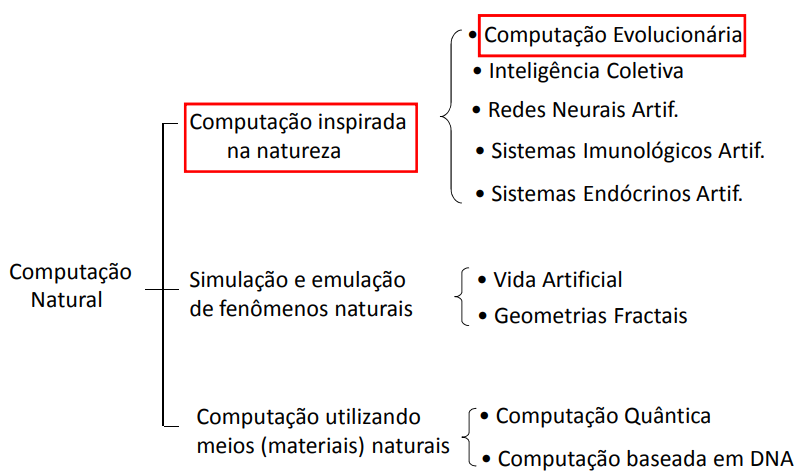
\includegraphics[width=.8\textwidth]{figuras/int_001}
	\caption[Computação Natural]{A Computação Natural possui três subdivisões, sendo elas computação inspirada na natureza ou algoritmos bio-inspirados (computação evolucionária, inteligência coletiva, redes neurais artificiais, sistemas imunológicos artificiais e sistemas endócrinos artificiais), simulação e emulação de fenômenos naturais (vida artificial e geometriais fractais) e a computação utilizando meios físicos naturais (computação quântica e computação baseada em DNA).}
	\ Fonte: \cite{pappa:2015:conceitos}. 
	\label{figura:int_001}
\end{figure}

\begin{figure}[htb]  
	\centering
	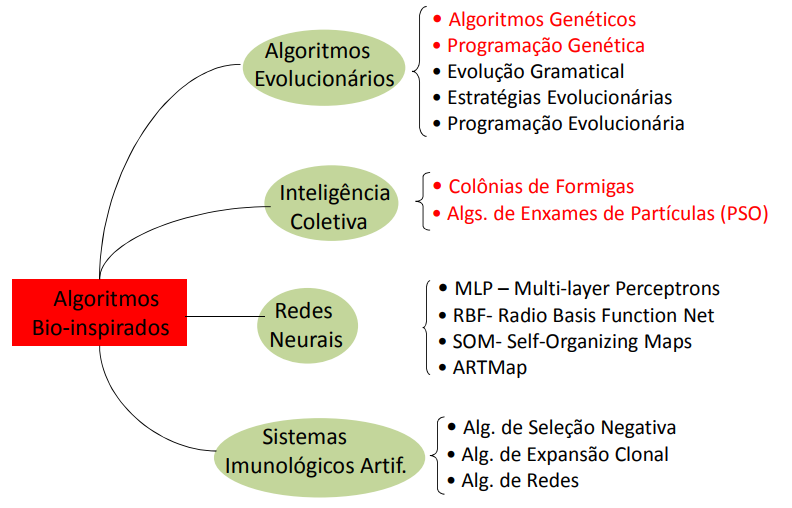
\includegraphics[width=.8\textwidth]{figuras/int_002}
	\caption[Algoritmos bio-inspirados]{Algoritmos bio-inspirados são divididos em: algoritmos evolucionários, inteligência coletiva, redes neurais e sistemas imunológicos artificiais.}
	\ Fonte: \cite{pappa:2015:conceitos}. 
	\label{figura:int_002}
\end{figure}

Além desses avanços, \citet{fuller:2011:computing} mostram que em função do ciclo virtuoso em que a tecnologia se encontra, a aplicação da computação em diversos outros sistemas podem ser vistos, como por exemplo, nos atuais \textit{smartphones}, smarTV's e sistemas embarcados que possuem componentes para computação de propósito geral e específico. Um destes modelos é o Raspberry Pi (basicamente é um pequeno computador) que possui processador, memória, comunicação com dispositivos de entrada e saída, entre outros.

Sendo assim, este trabalho apresenta o desenvolvimento de uma metodologia de comparação do desempenho de programas de forma sequencial e também de forma paralela em duas diferentes arquiteturas, ambas de propósito geral: plataforma Raspberry Pi e um computador \textit{desktop}. Vale ressaltar que o objetivo não é testar qual arquitetura é melhor em relação a outra, mas sim quão bom pode ser o desempenho de uma arquitetura embarcada se comparada ao de um computador comum.

\section{Objetivo Geral}
\label{subsecao:objetivo_geral}

Comparar o desempenho computacional paralelo e sequencial do Raspberry Pi em relação à computadores \textit{desktops}.

\subsection{Objetivos Específicos}
\label{subsecao:objetivos_especificos}

\begin{enumerate}
\item Definir o algoritmo a ser utilizado no trabalho a fim de utilizar o máximo possível do hardware em ambos os cenários.

\item Adaptar ou implementar o algoritmo para execução utilizando programação paralela.

\item Avaliar o desempenho computacional nas 2 arquiteturas propostas.
\end{enumerate}

\section{Justificativa}
\label{secao:justificativa}

Inicialmente, justifica-se esta pesquisa por demonstrar o uso de um computador de baixo custo que apresenta desempenho significativo e que está se tornando cada vez mais popular nos dias atuais, em comparação com um computador que já é utilizado. Outra justificativa é a carência de estudos comparativos de desempenho entre sistemas RISC e CISC. Além disso, fez-se a utilização de uma técnica que foi desenvolvida como solução para melhorar o desempenho dos processadores, que é a programação paralela, aproveitando todos os núcleos disponíveis. Como foi apresentado anteriormente, processadores \textit{multicore} são uma das soluções desenvolvidas para melhorar a capacidade de processamento visto que já não está sendo possível diminuir o tamanho físico dos transistores com a atual tecnologia de semicondutores. 

Assim, ressalta-se que em nossa instituição não há trabalhos científicos utilizando o Raspberry Pi, sendo assim este trabalho serve de alicerce para futuros trabalhos.

\section{Organização do Trabalho}
\label{secao:organizacao_trabalho}

Para um melhor entendimento desta monografia, o mesma foi dividida em capítulos. O capítulo 2 apresenta o referencial teórico, em que são descritos todos os termos e elementos necessários para uma melhor compreensão desta obra. O capítulo 3 apresenta a revisão de literatura, em que é mostrado o que existe de correlato, quais foram suas metodologias e resultados e, ao final como este trabalho se difere dos demais. O capítulo 4 apresenta os materiais e métodos utilizados para o desenvolvimento. Em outras palavras são descritas as técnicas e métricas utilizadas nesta produção. O capítulo 5 apresenta os resultados e discussões obtidos após a execução da metodologia descrita no capítulo 4 e faz uma comparação com os resultados da literatura descritos no capítulo 3. O capítulo 6 apresenta as conclusões obtidas com base nos resultados descritos no capítulo 5 e nos objetivos proposto no capítulo 1, quais limitações foram notadas, quais possíveis trabalhos futuros podem desenvolvidos. Por fim, o capítulo de referenciais apresenta a identificação e origem das obras consultadas para o desenvolvimento deste documento. 